\documentclass[aspectratio=169]{beamer}

\usepackage{cmap}

\usepackage[utf8]{inputenc}
\usepackage[english,russian]{babel}
\usepackage{fontspec}
\usepackage{tikz}

\usepackage{color}
\usepackage{listings}

\lstset{ %
    language=python,                % выбор языка для подсветки (здесь это С)
    basicstyle=\small\ttfamily,   % размер и начертание шрифта для подсветки кода
    numbers=left,                 % где поставить нумерацию строк (слева\справа)
    numberstyle=\tiny,            % размер шрифта для номеров строк
    stepnumber=1,                 % размер шага между двумя номерами строк
    firstnumber=1,
    numberfirstline=true
    numbersep=5pt,                % как далеко отстоят номера строк от подсвечиваемого кода
    backgroundcolor=\color{white},% цвет фона подсветки - используем \usepackage{color}
    showspaces=false,             % показывать или нет пробелы специальными отступами
    showstringspaces=false,       % показывать или нет пробелы в строках
    showtabs=false,               % показывать или нет табуляцию в строках
    frame=single,                 % рисовать рамку вокруг кода
    tabsize=2,                    % размер табуляции по умолчанию равен 2 пробелам
    captionpos=b,                 % позиция заголовка вверху [t] или внизу [b]
    breaklines=true,              % автоматически переносить строки (да\нет)
    breakatwhitespace=false      % переносить строки только если есть пробел
}

\usepackage{graphicx}
\usepackage{float}
\usepackage{subcaption}
\usepackage{xltabular, tabularx}

\setsansfont{Times New Roman}
\setmonofont{Consolas}

% no indent for itemize
\settowidth{\leftmargini}{\usebeamertemplate{itemize item}}
\addtolength{\leftmargini}{\labelsep}

\usetheme{metropolis}

\title{Сравнение методов сжатия атрибутов облаков точек}
\date{\today}
\author{Поздняков Артемий Анатольевич}
\institute{Высшая школа программной инженерии}
\begin{document}
  \newcommand{\Author}{Поздняков А. А.} % ФИО автора
\newcommand{\AuthorFull}{Поздняков Артемий Анатольевич} % ФИО автора
\newcommand{\Supervisor}{Фёдоров С. А.} % ФИО руководителя
\newcommand{\SupervisorFull}{Фёдоров Станислав Алексеевич}
\newcommand{\SupervisorPosition}{старший преподаватель ВШПИ ИКНК}
\newcommand{\ProfileCode}{09.03.04}
\newcommand{\ProfileName}{Программная инженерия}
\newcommand{\ConsultantNorm}{Локшина Е. Г.} %ФИО нормконтроль
\newcommand{\TaskCreatedBukvami}{''18'' апреля 2024 г.}
\newcommand{\TaskCreatedCiframi}{18.04.2024}
\newcommand{\TaskDeadline}{20.05.2024}

\newcommand{\Theme}{Сравнение методов сжатия атрибутов облаков точек} %тема диплома
\newcommand{\Group}{5130904/00104} %группа


  \begin{frame}[noframenumbering, plain]

    \begin{center}
      \begin{scriptsize}
        Министерство науки и высшего образования Российской Федерации\\
        Санкт-Петербургский политехнический университет Петра Великого\\
        Институт компьютерных наук и кибербезопасности\\
        Высшая школа программной инженерии\\[5\baselineskip]
      \end{scriptsize}

      \Large\textbf{\Theme{}}
    \end{center}

    \begin{flushright}
      \begin{scriptsize}
        Выполнил студент: \textbf{\AuthorFull{}}, гр. \Group{}\\
        Научный руководитель: \SupervisorPosition{} \textbf{\SupervisorFull{}}\\
        Направление подготовки: \ProfileCode{}, \textbf{\ProfileName{}}\\
      \end{scriptsize}
    \end{flushright}

    \mbox{}\vfill

    \begin{center}
      \begin{scriptsize}
        Санкт-Петербург \\
        \the\year{}
      \end{scriptsize}
    \end{center}

    \begin{tikzpicture}[remember picture, overlay]
      \node[xshift=1mm, yshift=-1mm, anchor=north west] at (current page.north west){%
        
\includegraphics[width=20mm]{assets/heraldic.png}};
    \end{tikzpicture}

  \end{frame}

  \setcounter{framenumber}{2}

  \begin{frame}{Актуальность}
    Разработка программы для оценки работы PCC-кодеков - актуальная задача.

    \begin{itemize}
      \item Популярность технологий компьютерного зрения и расширенной
      реальности растёт;
      \item Появляется большое количество кодеков, предназначенных для сжатия
      облаков точек и их атрибутов (PCC-кодеков);
    \end{itemize}

    \metroset{block=fill}
    \begin{block}{Использование}
      Подобная программа может быть использована исследователями для подсчёта
      метрик разрабатываемых ими кодеков.
    \end{block}
  \end{frame}

  \begin{frame}{Цели и задачи}

  \textbf{Цель работы} - разработка подхода к сравнению методов сжатия атрибутов
  облаков точек.

  Задачи:

  \begin{itemize}
      \item Проанализировать системы оценки качества сжатия облаков точек;
      \item Изучить релевантные метрики, отображающие эффективность и качество
      сжатия атрибутов облаков точек;
      \item Разработать программу подсчёта метрик;
      \item Получить метрики для отобранных PCC-кодеков;
      \item Проанализировать результаты работы;
  \end{itemize}

  \end{frame}

  \begin{frame}{Оценка качества сжатия}
    \metroset{block=fill}
    \begin{block}{Определение}
      Реконструированное облако - облако точек, полученное в результате
      компрессии и декомпрессии оригинального облака точек.
    \end{block}

    \begin{itemize}
      \item Показателем качества сжатия являются значения отобранных метрик для
      пары оригинальное и реконструированное облако.
    \end{itemize}
  \end{frame}

  \begin{frame}{Сравнение альтернативных решений}
    \begin{table}
      \begin{xltabular}{\linewidth}{|l|X|X|}
        \hline
        & mpeg\_pcc\_dmetric & geo\_dist \\
        \hline
        Полнота метрик & ± & ± \\
        \hline
        Оценка искажения атрибутов & + & - \\
        \hline
        Поддерживаемость & + & - \\
        \hline
        Возможность расширения & - & - \\
        \hline
        Открытый исх. код & - & - \\
        \hline
      \end{xltabular}
      \caption{
          Характеристики различных рассмотренных систем
      }
    \end{table}
  \end{frame}

  \begin{frame}{Требования}
    В результате анализа определены следующие требования к разрабатываемому
    решению:

    \begin{itemize}
        \item Возможность вычисления стандартных метрик искажения геом.
        структуры (MSE и PSNR, метрика Хаусдорфа);
        \item Возможность вычисления проецированных значений отклонения;
        \item Возможность вычисления искажения цветов в цветовых схемах RGB и Y'CbCr;
        \item Использование архитектуры, допускающей дальнейшее расширение
        приложения;
        \item Наличие тестов;
        \item Использование лицензии MIT;
    \end{itemize}
  \end{frame}

  \begin{frame}{Архитектура разрабатываемого решения}
    \begin{figure}[H]
        \centering
        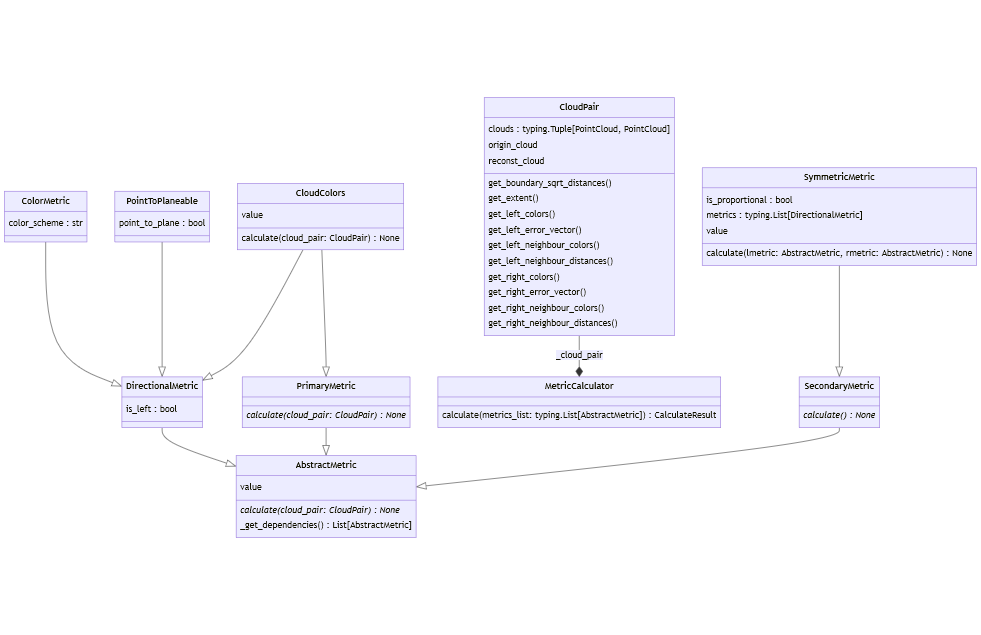
\includegraphics[width=\linewidth]{assets/classes.png}
        \caption{Диаграмма классов разработанного приложения}
        \label{img:metric_classes}
    \end{figure}
  \end{frame}

  \begin{frame}[fragile]{Алгоритм внедрения зависимостей}
    \begin{lstlisting}[caption={
      Алгоритм внедрения зависимостей
    }, label={lst:calculator_recursive_calculate},
    basicstyle=\tiny\ttfamily,
    gobble=6]
      if metric._key() in self._calculated_metrics:
          return self._calculated_metrics[metric._key()]

      if isinstance(metric, PrimaryMetric):
          metric = typing.cast(PrimaryMetric, metric)
          metric.calculate(self._cloud_pair)
          self._calculated_metrics[metric._key()] = metric
          return metric

      calculated_deps = {}
      for dep_key, dep_metric in metric._get_dependencies().items():
          calculated_dep_metric = self._metric_recursive_calculate(
              metric=dep_metric,
          )
          calculated_deps[dep_key] = calculated_dep_metric

      metric.calculate(**calculated_deps)
      self._calculated_metrics[metric._key()] = metric
    \end{lstlisting}
  \end{frame}

  \begin{frame}{Консольное приложение}
    \begin{figure}[H]
        \centering
        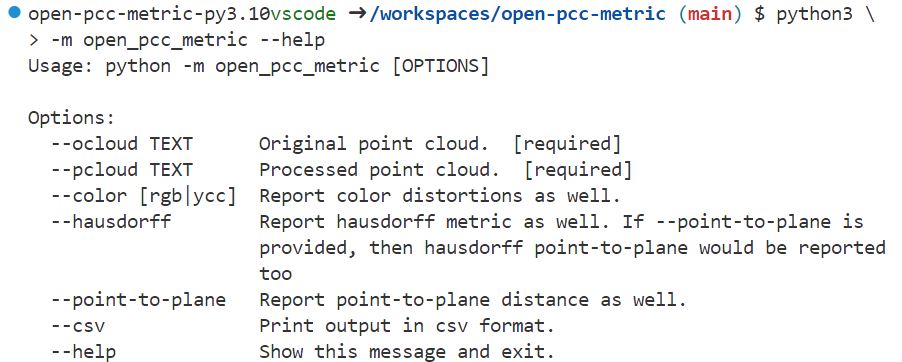
\includegraphics[width=0.9\linewidth]{assets/open_pcc_metric_help.png}
        \caption{Help-сообщение программы}
        \label{img:pcc_metric_help}
    \end{figure}
  \end{frame}

  \begin{frame}{Консольное приложение}
    \begin{figure}[H]
        \centering
        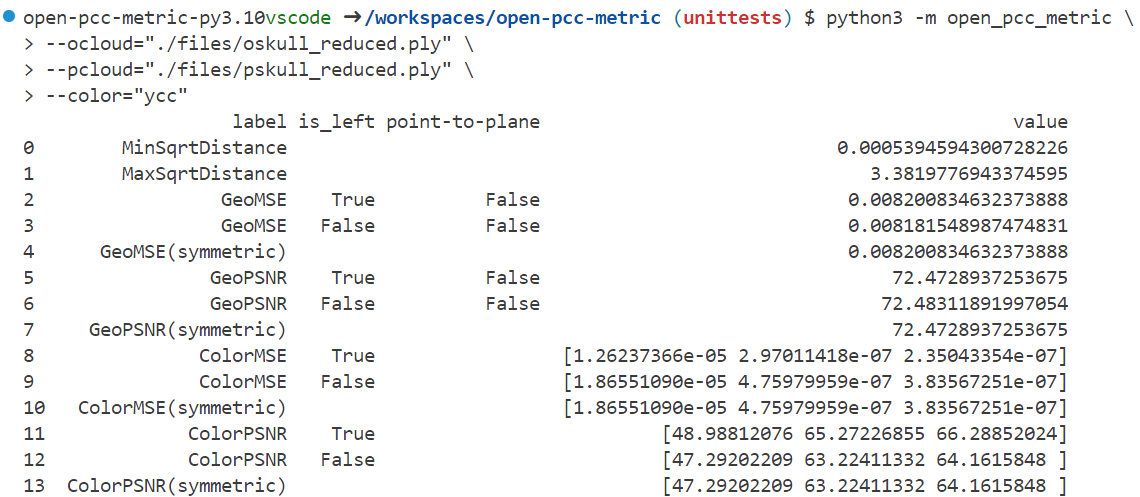
\includegraphics[width=0.9\linewidth]{assets/open_pcc_metric_output.png}
        \caption{Пример вывода программы}
        \label{img:pcc_metric_output}
    \end{figure}
  \end{frame}

  \begin{frame}{Детали реализации}
    \vspace{\baselineskip}
    % Тут про объем реализации (1к строк кода), тесты, CI/CD, много картинок, пару
    % красивых слов.
    \begin{columns}
      \column{0.2\linewidth}
        \begin{scriptsize}
          Стек:
          \begin{itemize}
            \item Python 3.8.1
            \item Open3D 0.18.0
            \item NumPy 1.24
            \item click 8.1.7
          \end{itemize}
          Линтеры:
          \begin{itemize}
            \item pylint
            \item flake8
          \end{itemize}
          Тестирование:
          \begin{itemize}
            \item pytest
          \end{itemize}
          CI/CD:
          \begin{itemize}
            \item GitHub Actions
          \end{itemize}
          Объем реализации:
          \begin{itemize}
            \item 1206 строк
          \end{itemize}
        \end{scriptsize}
      \column{0.7\linewidth}
        \scalebox{0.8}{
          \begin{minipage}{1.20\textwidth}
            \begin{figure}
              \centering
              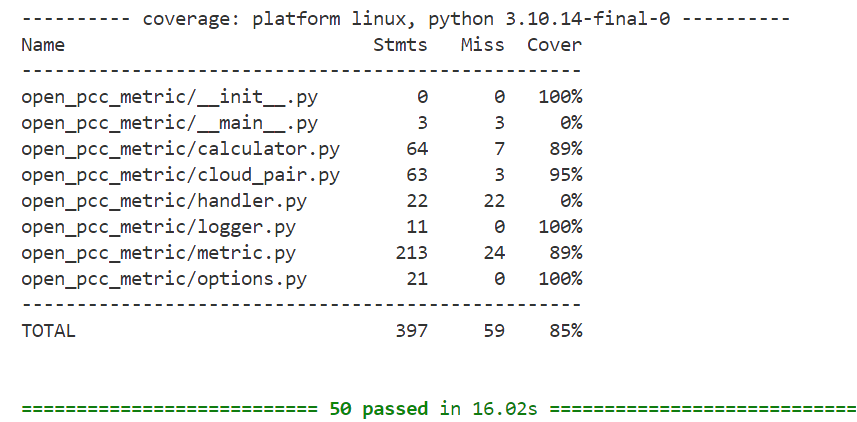
\includegraphics[width=0.7\linewidth]{assets/coverage.png}
              \caption{Покрытие тестами}
            \end{figure}
            \vspace{-1\baselineskip}
            \begin{figure}
              \centering
              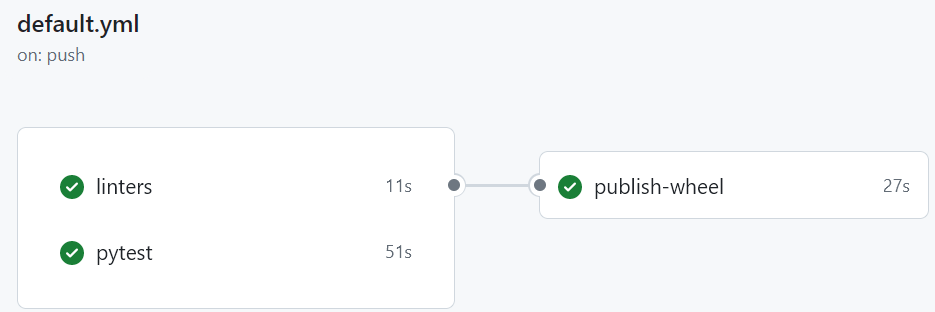
\includegraphics[width=0.7\linewidth]{assets/actions_status.png}
              \caption{Статус CI/CD}
            \end{figure}
          \end{minipage}
        }
    \end{columns}
  \end{frame}

  \begin{frame}{PCCArena}
    \begin{columns}
      \column{0.38\linewidth}
        PCCArena - система бенчмаркинга PCC-кодеков. Данная система использует
        mpeg\_pcc\_dmetric для вычисления стандартных метрик (MSE, PSNR, и
        т.д.).
       \column{0.58\linewidth}
        \begin{figure}
          \centering
          
\includegraphics[width=\linewidth]{assets/pcc_arena_github.jpg}
          \caption{Репозиторий PCCArena на GitHub}
        \end{figure}
     \end{columns}

  \end{frame}

  \begin{frame}{Архитектура PCCArena}
    \begin{figure}[H]
        \centering
        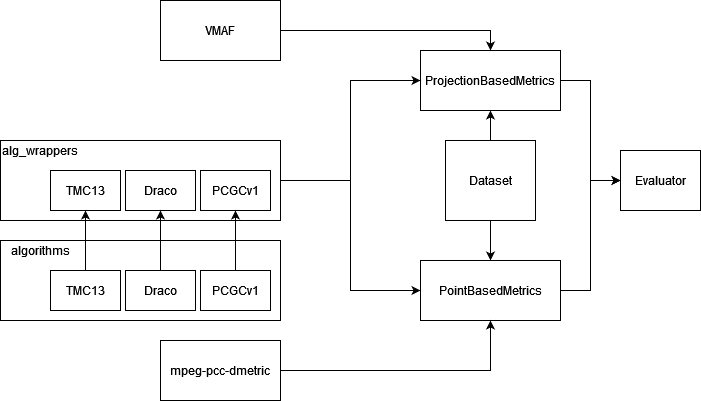
\includegraphics[width=0.7\linewidth]{assets/pcc_arena_architecture.png}
        \caption{Архитектура PCCArena}
        \label{img:pcc_arena_architecture}
    \end{figure}
  \end{frame}

  \begin{frame}{Описание проведенных экспериментов}
    С помощью модифицированной системы PCCArena был произведен набор измерений.

    \begin{itemize}
      \item Произведена оценка кодеков TMC13 и Draco;
      \item Использовался датасет ShapeNet;
      \item Для каждой метрики была построена зависимость от битрейта;
    \end{itemize}

    \metroset{block=fill}
    \begin{block}{Определение}
      Битрейт - количество бит, затраченных на кодирование одной точки.
    \end{block}
  \end{frame}

  \begin{frame}{Результаты для расстояния Чамфера}
    \begin{figure}[H]
        \centering
        \begin{subfigure}{0.49\textwidth}
            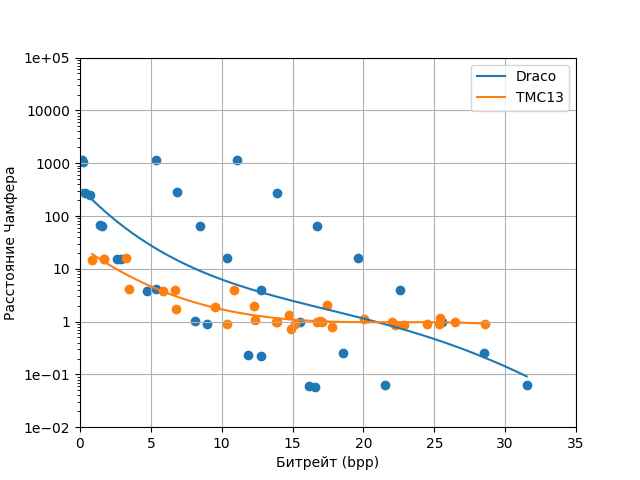
\includegraphics[width=\linewidth]{assets/approx_cd_p2pt.png}
            \caption{}
        \end{subfigure}
        \begin{subfigure}{0.49\textwidth}
            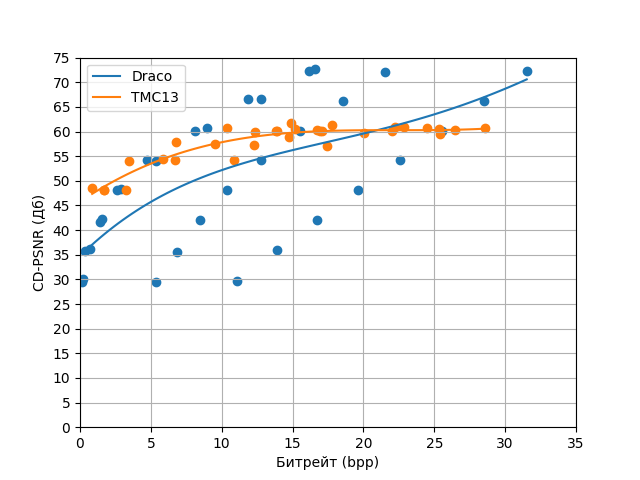
\includegraphics[width=\linewidth]{assets/approx_cdpsnr_p2pt.png}
            \caption{}
        \end{subfigure}
        \caption{ (a) Зависимость расстояния Чамфера от битрейта. (b) Зависимость
        CD-PSNR от битрейта }
        \label{img:pcc_arena_cd_bpp}
    \end{figure}
  \end{frame}

  \begin{frame}{Результаты для метрики Хаусдорфа и нормалей}
    \begin{figure}[H]
        \centering
        \begin{subfigure}{0.49\textwidth}
            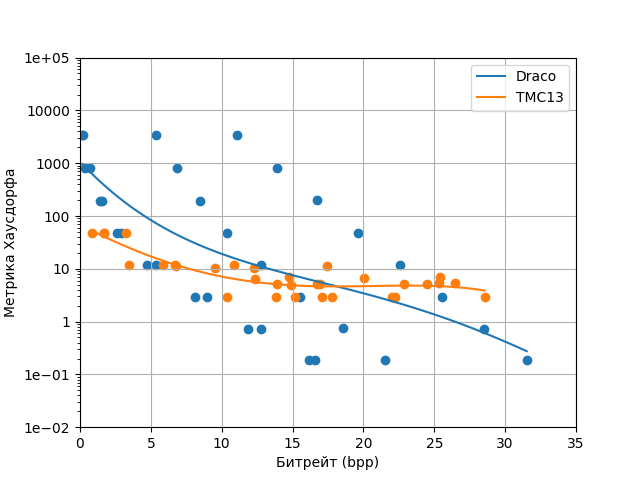
\includegraphics[width=\linewidth]{assets/approx_h_p2pt.png}
            \caption{}
        \end{subfigure}
        \begin{subfigure}{0.49\textwidth}
            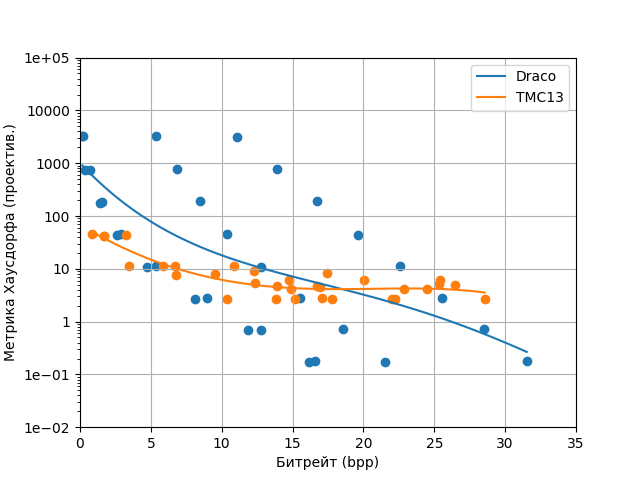
\includegraphics[width=\linewidth]{assets/approx_h_p2pl.png}
            \caption{}
        \end{subfigure}
        \caption{ (a) Зависимость метрики Хаусдорфа от битрейта. (b) Зависимость
        проецированной метрики Хаусдорфа от битрейта }
        \label{img:pcc_arena_hd}
    \end{figure}
  \end{frame}

  \begin{frame}{Результаты для цветов}
    \begin{figure}[H]
        \centering
        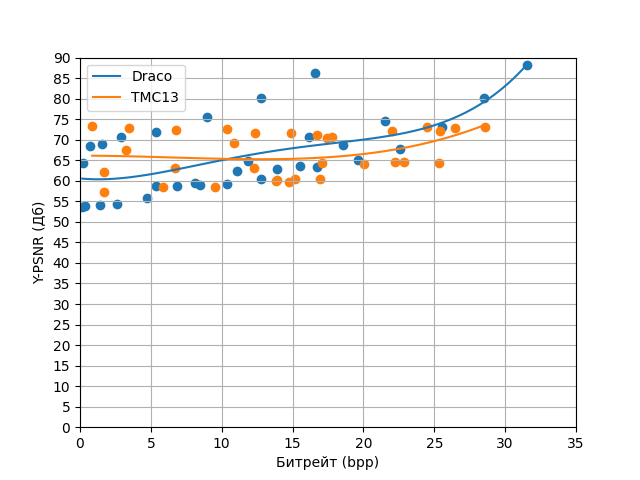
\includegraphics[width=0.49\linewidth]{assets/approx_y_psnr.png}
        \caption{ Зависимость Y'-PSNR от битрейта }
        \label{img:pcc_arena_y_psnr}
    \end{figure}
  \end{frame}

  \begin{frame}{Выводы и дальнейшие шаги}
    \begin{itemize}
      \item Проведён анализ существующих систем оценки методов сжатия облаков
      точек и их атрибутов;
      \item Разработана программа для оценки качества облака точек при наличии
      оригинального облака точек;
      \item Произведён сравнительный анализ кодеков Draco и TMC13;
    \end{itemize}

    Разработанное решение упростит оценку методов сжатия атрибутов облаков точек
    и может быть полезно исследователям, ведущим разработки в данной области.

    Дальнейшие шаги:

    \begin{itemize}
      \item Могут быть добавлены метрики, учитывающие более высокоуровневые
      признаки облаков точек и дающие более подробную оценку качества их сжатия;
    \end{itemize}
  \end{frame}
\end{document}